%preamble
\documentclass[letterpaper]{article}
\synctex=1

\usepackage{geometry}
\usepackage{array}
\usepackage{lipsum}

\usepackage{graphicx}
\usepackage{float}
\graphicspath{ {images/} }

\usepackage{float}

\usepackage[hidelinks]{hyperref}

\usepackage{xcolor}
% \usepackage[section]{placeins}
%
% \newenvironment{changemargin}[2]{%
% \begin{list}{}{%
% \setlength{\topsep}{0pt}%
% \setlength{\leftmargin}{#1}%
% \setlength{\rightmargin}{#2}%
% \setlength{\listparindent}{\parindent}%
% \setlength{\itemindent}{\parindent}%
% \setlength{\parsep}{\parskip}%
% }%
% \item[]}{\end{list}}

% \usepackage{tabu}
%actual document
\begin{document}

%titlepage
\begin{titlepage}
 \begin{center}

  \LARGE
  ECE 321 Lab\\ Software Requirements Engineering
  
  Department of Electrical and Computer Engineering\\
  
  University of Alberta
  
  \vspace{2cm}
  
  404 Team Name Not Found
  
  \vspace{5cm}
  \Large
  
  \begin{tabular}{ | m{5cm} | m{5cm} | }
   \hline
   Student Name  & Student \\
   \hline
   Arun Woosaree & XXXXXX  \\
   \hline
   Max           & XXXXXX  \\
   \hline
   Liyao         & XXXXXX  \\
   \hline
  \end{tabular}
  
  
  % \begin{tabu} to 0.8\textwidth{  | X[c] | X[c] | }
  %   \hline
  %   Student Name & Student \\
  %   \hline
  %   Arun Woosaree & xxxxxxx \\
  %   \hline
  %   Navras Kamal & 1505463 \\
  %   \hline
  % \end{tabu}
  
  
 \end{center}
\end{titlepage}

%table of contents
\tableofcontents
\vfill
\newpage

\section{Customer:}
Client:
Alberta Traffic Supply Ltd.\\
7798 16 th Street\\
Edmonton, Alberta, T6P 1L9\\
Western Canada largest traffic sign manufacture and traffic control company\\

\section{Definitions}
\label{Definitions}
\begin{figure}[h!]
 \centering
 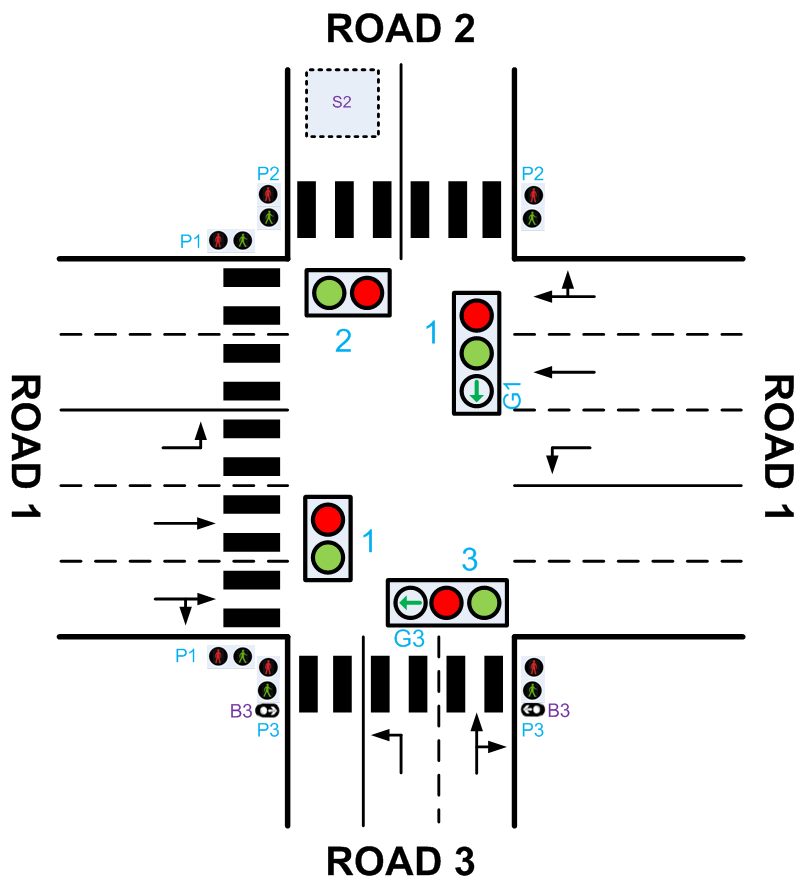
\includegraphics[width=\textwidth]{intersection.png}
 \caption{INSERT CAPTION HERE}
 \label{intersection}
\end{figure}

\textit{Labels}
\textbf{1,2,3,P1,P2,P3,B3,S2,G1,G3}
\textit{can be found in Figure \ref{intersection}.}
\begin{enumerate}

 \item \textbf{TLMS} -
       \textbf{T}raffic
       \textbf{L}ight
       \textbf{M}onitoring
       \textbf{S}ystem
       
 \item \textbf{RB} -
       \textbf{R}eset
       \textbf{Button}
 \item \textbf{M} - Hardware malfunction: 1 indicates a malfunction, 0 for normal operation
 \item \textbf{1} - Light on Road 1
 \item \textbf{2} - Light on Road 2
 \item \textbf{3} - Light on Road 3
 \item \textbf{P1} - Pedestrian light on road 1
 \item \textbf{P2} - Pedestrian light on road 2
 \item \textbf{P3} - Pedestrian light on road 3
 \item \textbf{t1} - Timer for \textbf{1}
 \item \textbf{t2} - Secondary timer for everything else
 \item \textbf{G1} - Left turn signal on road 1
 \item \textbf{G3} - Left turn signal on road 3
 \item \textbf{S2} - Magnetic sensor which detects if a car/motorcycle is waiting on \textbf{2}\\
       Outputs: 1 if vehicle waiting, 0 otherwise
 \item \textbf{B3} - Button on road 3 which a pedestrian can hit to request to cross the intersection
 \item \textbf{BG} -
       \textbf{B}linking
       \textbf{G}reen
 \item \textbf{BR}
       \textbf{B}linking
       \textbf{R}ed
 \item \textbf{D} - \textbf{D}ay (6:00-20:00)
 \item \textbf{N} - \textbf{N}ight (20:00-6:00)
 \item \textbf{Clock} - Can have value \textbf{D} or \textbf{N}
 \item \textbf{}
 \item \textbf{}
       
       
\end{enumerate}


\section{Description}
Lorem ipsum dolor sit amet, consectetur adipiscing elit, sed do eiusmod tempor
incididunt ut labore et dolore magna aliqua. Ut enim ad minim veniam, quis
nostrud exercitation ullamco laboris nisi ut aliquip ex ea commodo consequat.
Duis aute irure dolor in reprehenderit in voluptate velit esse cillum dolore eu
fugiat nulla pariatur. Excepteur sint occaecat cupidatat non proident, sunt in
culpa qui officia deserunt mollit anim id est laborum.
road \textbf{1} is main, \textbf{3} is also main but \textbf{1} is the most important, and
road \textbf{2} is secondary


\section{Requirements}
\begin{enumerate}
 \item The software will be running on imbedded system with 550KB hard drive, 50KB RAM.
 \item The software desgin should obey regulations on traffic lights posted by Canadian Transportation Agency.
 \item The software desgin should focus on safety, reliability and correctness. The system should be up as much as possible.
 \item The software should use different timers. Timer 1 is used for road 1 only, and timer 2 is used for the rest.
 \item Road 1 and 3 are main roads, and road 2 is secondary. Priority should be given in the sequence of road 1, road 3, road 2.
 \item Pedestrian lights should turn green when it is safe to cross.
 \item System should go to emergency state when there is a hardware malfunction, and go back to default mode when exiting emergency state.
 \item The system should have a physical button for reset. During a reset, the system should go to emergency mode first, and then the default mode.
 \item The system should be tested using emulations. It should also demonstrate satisfactory performance before puting in use.
\end{enumerate}

\section{Nice-to-haves}
\begin{enumerate}
 \item Data logging system, but design should account for the limited storage.
 \item Indication of which part of the system is malfunctioning.
 \item Configurable timing for traffic flow optimization purpose.
 \item Protection of the sensor S2.
\end{enumerate}



\section{State description}
\textbf{Note: }
\begin{itemize}
 \item \textit{Labels}
       \textbf{1,2,3,P1,P2,P3,B3,S2,G1,G3}
       \textit{are defined on page \pageref{Definitions} and in Figure \ref{intersection} on page \ref{intersection}.}
 \item {\color{green}Green} and {\color{red}Red} text indicate what colour the light should be in the respective state
\end{itemize}

\begin{enumerate}
 \item \textbf{Default}
       \begin{itemize}
        \item {\color{green}\textbf{1,P2}}
        \item {\color{red}\textbf{2,3,P1,P3,G1,G3}}
        \item \textbf{t1} activated
        \item \textbf{M}: 0
        \item \textbf{Clock}: \textbf{D}
       \end{itemize}
 \item \textbf{Green G1}
       \begin{itemize}
        \item {\color{green}\textbf{G1,P1}}
        \item {\color{red}\textbf{1,2,3,P2,P3,G3}}
        \item \textbf{t2} activated
        \item \textbf{M}: 0
        \item \textbf{Clock}: \textbf{D}
       \end{itemize}
       Note:
       \begin{enumerate}
        \item \textbf{Green G1 S2} \textit{is this state, but when} \textbf{S2}=1
       \end{enumerate}
       
       
 \item \textbf{Green 3}
       \begin{itemize}
        \item {\color{green}\textbf{3,G3}}
        \item {\color{red}\textbf{1,2,P1,P2,P3,G1}}
        \item \textbf{t2} activated
        \item \textbf{M}: 0
        \item \textbf{Clock}: \textbf{D}
       \end{itemize}
       Note:
       \begin{enumerate}
        \item \textbf{Green 3 S2} \textit{is this state, but when} \textbf{S2}=1
       \end{enumerate}
 \item \textbf{Green P3}
       \begin{itemize}
        \item {\color{green}\textbf{1,P2,P3}}
        \item {\color{red}\textbf{2,3,P1,G1,G3}}
        \item \textbf{t2} activated
        \item \textbf{M}: 0
        \item \textbf{Clock}: \textbf{D}
       \end{itemize}
       Note:
       \begin{enumerate}
        \item \textbf{Green P3 S2} \textit{is this state, but when} \textbf{S2}=1
       \end{enumerate}
 \item \textbf{Green 2\&3}
       \begin{itemize}
        \item {\color{green}\textbf{2,3}}
        \item {\color{red}\textbf{1,P1,P2,P3,G1,G3}}
        \item \textbf{t2} activated
        \item \textbf{M}: 0
        \item \textbf{Clock}: \textbf{D}
       \end{itemize}
 \item \textbf{Night}
       \begin{itemize}
        \item {\color{green}\textbf{1}} \textbf{BG}
        \item {\color{red}\textbf{2,3}} \textbf{BR}
        \item \textbf{P1,P2,P3,G1,G3} are turned off
        \item \textbf{M}: 0
        \item \textbf{Clock}: \textbf{N}
       \end{itemize}
 \item \textbf{Emergency}
       \begin{itemize}
        \item {\color{green}\textbf{1}} \textbf{BG}
        \item {\color{red}\textbf{2,3}} \textbf{BR}
        \item \textbf{P1,P2,P3,G1,G3} are turned off
        \item \textbf{M}: 1
        \item \textbf{Clock}: \textbf{D} or \textbf{N}
       \end{itemize}
       Note:
       \begin{enumerate}
        \item When the system first starts up, it should briefly go into emergency mode
              with \textbf{M}=0 then immediately switch to default mode.
              (Because hardware malfunctions should be fixed before the system starts.)
       \end{enumerate}
\end{enumerate}

\begin{figure}[H]
 \centering
 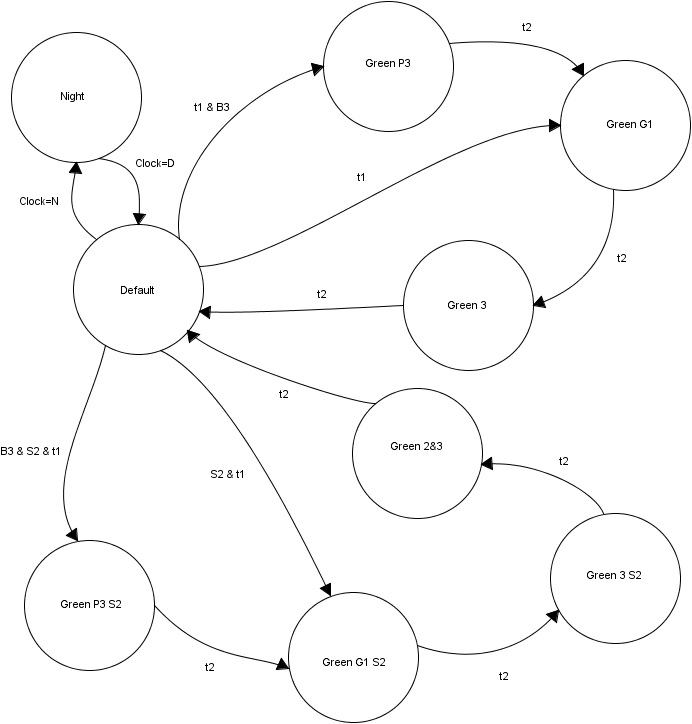
\includegraphics[width=\textwidth]{fsm.jpg}
 \caption{INSERT CAPTION HERE}
 \label{fsm}
\end{figure}

\section{Special considerations}

\begin{enumerate}
 \item Security\\
       Here's how we make the system more secure:
       \begin{enumerate}
        \item step 1
        \item step 2
        \item step 3
       \end{enumerate}
 \item Reliability
 \item Synced timings
\end{enumerate}


\end{document}
